\documentclass{article}
\usepackage{amsmath}
\usepackage{tikz}
\usepackage[a4paper]{geometry}
\usepackage{fancyhdr}
\pagestyle{fancy}
\lhead{Mechanische Schwingungen}
\rhead{September 2025}
\begin{document}
\section{Mechanische Schwingungen}
Eine Schwingung ist eine zeitlich periodische Änderung einer physikalischen Größe, welche nach einer einmaligen Auslenkung aus der Ruhelage anfängt, verursacht durch rücktreibende Kräfte.
 
Schwingungen werden durch ihre \emph{Periodendauer} $T$, ihre \emph{Frequenz} $f$ in $\text{Hz}$ mit $f=\dfrac{1}{T}$ und ihre \emph{Amplitude} $y_{max}$ beschrieben. Die zurzeitige Auslenkung, $y(t)$, wird die \emph{Elongation} genannt.
\begin{center}
 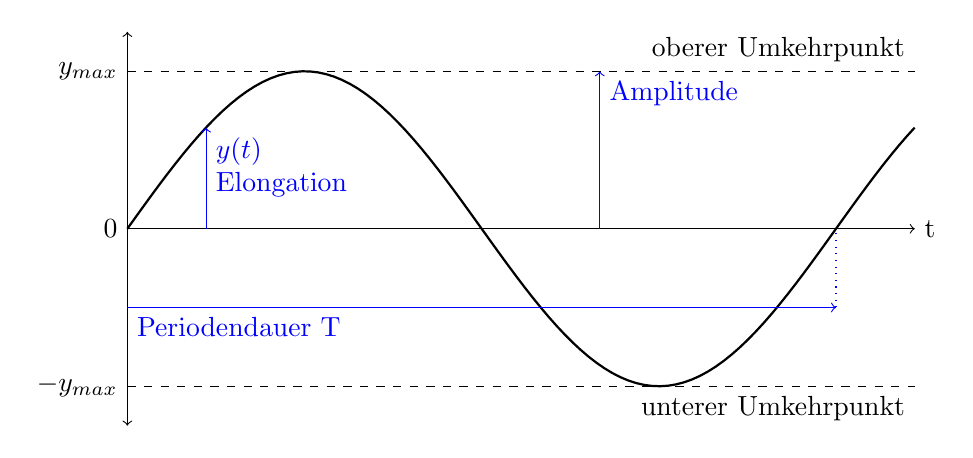
\begin{tikzpicture}     
  \draw[thick, domain=0:10, samples=100] 
            plot (\x, {2*sin(\x*360 / 9)});
     
  \draw[->] (0, 0) -- (10, 0) node[right] {t};
  
  \draw (0, 0) node[left] {$0$}; 
  \draw (0, 2) node[left] {$y_{max}$}; 
  \draw (0, -2) node[left] {$-y_{max}$};
  \draw[<->] (0, -2.5) -- (0, 2.5); 
  
  \draw[->, blue] (1, 0) -- (1, {2*sin(1*360/9)}) node[below right, align=left] {$y(t)$ \\ Elongation};  
  \draw[->, blue] (6, 0) -- (6, 2) node[below right] {Amplitude};  
  \draw[->, blue] (0, -1) node[below right] {Periodendauer T} -- (9, -1);
  \draw[dotted, blue] (9, -1) -- (9, 0);
 
  \draw[dashed] (0, 2) -- (10, 2) node[above left] {oberer Umkehrpunkt};
  \draw[dashed] (0, -2) -- (10, -2) node[below left] {unterer Umkehrpunkt};  
 \end{tikzpicture} 
\end{center} 
 
\subsection{Harmonische Schwingungen} 
Eine Schwingung ist eine \emph{harmonische Schwingung}, wenn sie
\begin{enumerate}
 \item durch eine Sinusfunktion beschrieben werden kann
 \item auf eine gleichförmige Kreisbewegung zurückgeführt werden kann
 \item eine zeitlich konstante Schwingungsdauer hat 
 \item auf einer rücktreibenden Kraft, welche zur Elongation proportional ist, basiert 
\end{enumerate} 
Diese vier Bedingungen sind eigentlich equivalent zueinander, wenn eine erfüllt ist, dann sind alle erfüllt.
 
\subsection{Quantitativ}
Die generelle Schwingungsgleichung $y(t)$ ist, in RAD
\[
 y(t) = y_{max} \cdot \sin{\left(\frac{2\pi}{T} \cdot t\right)}
\]
Diese Formel kann so begründet werden, dass nach einer ganzen Periode, also wenn $t=T$, $y(T)=0$ sein sollte, wobei bei einer Sinusfunktion $\sin{(k \cdot 2\pi)} = 0$ für ein ganzzahliges $k$ ist. Somit muss innerhalb des Sinus mit $2\pi / T$ multipliziert werden, damit $2\pi \cdot t/T$ bei $t=T$ zu $2\pi$, der Periodenlänge einer Sinusfunktion in RAD, wegfällt. \newline
Der Vorfaktor $y_{max}$ wird genutzt, damit der Wertebereich einer normalen Sinusfunktion von $[-1; 1]$ zu dem gewollten $[-y_{max}; y_{max}]$ multipliziert wird. 
\end{document}